\documentclass[11pt,a4paper]{article}
\usepackage[utf8]{inputenc}
\usepackage{graphicx}
\usepackage{multirow}
\usepackage{enumitem}
\usepackage{amsmath,amssymb}
\usepackage{array}
\usepackage{xcolor}
\usepackage{tikz}
\usepackage{pgfplots}
\usetikzlibrary{arrows.meta}
\pgfplotsset{compat=1.18}
\usepackage[left=15mm,right=15mm,top=12mm,bottom=12mm]{geometry}
\graphicspath{{C:/Users/teoso/Documents/Template Math Depart/}}
\newcommand{\R}{\mathbb{R}}
\setlength{\parindent}{0pt}
\setlist[enumerate,1]{label=\arabic*.,leftmargin=*,itemsep=8pt,parsep=3pt,topsep=6pt}
\setlist[enumerate,2]{label=(\alph*),leftmargin=*,itemsep=7pt,parsep=3pt,topsep=5pt}

\begin{document}
\pagenumbering{gobble}
\setlength{\abovedisplayskip}{7pt}
\setlength{\belowdisplayskip}{7pt}
\setlength{\abovedisplayshortskip}{4pt}
\setlength{\belowdisplayshortskip}{4pt}

\noindent
\begin{minipage}{0.14\textwidth}
  \includegraphics[width=1.8cm]{ITS.png}
\end{minipage}%
\begin{minipage}{0.72\textwidth}
  \centering
  \textbf{EVALUASI TENGAH SEMESTER GASAL 2025/2026}\\
  \textbf{DEPARTEMEN MATEMATIKA -- FSAD ITS}
\end{minipage}%
\begin{minipage}{0.14\textwidth}
  \centering
  \includegraphics[width=1.6cm]{M.png}
\end{minipage}

\vspace{0.25cm}
\begin{center}
  \begin{tabular}{@{}l c l@{}}
    Mata Kuliah/Kode & : & Kalkulus Peubah Banyak                   \\
    Hari/Tanggal     & : & Rabu, 15 Oktober 2025                    \\
    Sifat/Waktu      & : & Tutup Buku / 100 menit                   \\
    Dosen            & : & Dra. Nur Asiyah, M.Si. (A)               \\
                     &   & Dr. Didik Khusnul Arif, S.Si., M.Si. (D) \\
                     &   & Drs. Lukman Hanafi, M.Sc. (C)            \\
                     &   & Drs. Kamiran, M.Si. (B)
  \end{tabular}
\end{center}

\noindent\fbox{\parbox{\dimexpr\textwidth-2\fboxsep-2\fboxrule\relax}{%
    \textbf{HARAP DIPERHATIKAN !!!}\\
    \textit{Segala jenis pelanggaran (mencontek, kerjasama, dsb) yang dilakukan saat ETS/EAS
      akan dikenakan sanksi pembatalan mata kuliah pada semester yang sedang berjalan.}
  }}

\vspace{0.2cm}
ETS mengukur kemampuan
\begin{center}
  \small
  \setlength{\tabcolsep}{5pt}
  \renewcommand{\arraystretch}{1.1}
  \begin{tabular}{|>{\centering\arraybackslash}p{1.6cm}|>{\raggedright\arraybackslash}p{\dimexpr\textwidth-5.15cm-12\tabcolsep-7\arrayrulewidth\relax}|>{\centering\arraybackslash}p{1.9cm}|*{3}{>{\centering\arraybackslash}p{0.55cm}|}}
    \hline
    \multirow{2}{*}{CPMK} & \multirow{2}{*}{ETS mengukur kemampuan}
                          & \multirow{2}{*}{\shortstack{Bobot\\CPMK (\%)}}
                          & \multicolumn{3}{c|}{CPL}                                                                                                                                                                                       \\ \cline{4-6}
                          &                                                                                                                                                               &              & 5            & 7            & 9 \\ \hline
    CPMK-1                & Mahasiswa mampu memahami dan mampu menjelaskan fungsi dengan dua peubah dan dapat mensketsa grafik fungsinya
                          & 8\%                                                                                                                                                           & $\checkmark$ &              &                  \\ \hline
    CPMK-2                & Mahasiswa mampu memahami dan mampu menjelaskan konsep limit, kekontinuan, diferensiasi dan integrasi untuk fungsi peubah banyak
                          & 7\%                                                                                                                                                           & $\checkmark$ &              &                  \\ \hline
    CPMK-3                & Mahasiswa mampu mengaplikasikan turunan fungsi lebih dari satu peubah terhadap masalah maksimum dan minimum serta dapat memberikan contoh dalam fenomena riil
                          & 10\%                                                                                                                                                          & $\checkmark$ & $\checkmark$ & $\checkmark$     \\ \hline
  \end{tabular}
\end{center}

\begin{center}
  \small
  \renewcommand{\arraystretch}{1.05}
  \begin{tabular}{|c|c|*{3}{>{\centering\arraybackslash}p{2.3cm}|}}
    \hline
    \multicolumn{5}{|c|}{ETS Mengukur Capaian Pembelajaran Mata Kuliah}                                  \\ \hline
    \multirow{2}{*}{Soal nomor}            & \multirow{2}{*}{Bobot Soal (\%)}
                                           & \multicolumn{3}{c|}{Bobot CPMK}                             \\ \cline{3-5}
                                           &                                  & CPMK 1 & CPMK 2 & CPMK 3 \\ \hline
    1                                      & 25                               &        & 4      &        \\ \hline
    2                                      & 25                               & 8      &        &        \\ \hline
    3                                      & 25                               &        & 3      &        \\ \hline
    4                                      & 25                               &        &        & 10     \\ \hline
    \multicolumn{2}{|l|}{TOTAL BOBOT CPMK} & 8                                & 7      & 10              \\ \hline
  \end{tabular}
\end{center}

\begin{enumerate}[itemsep=6pt,parsep=0pt]
  \item \begin{enumerate}[label=\alph*.,itemsep=5pt,topsep=0pt]
          \item Tunjukkan bahwa
                $\displaystyle\lim_{(x,y)\to(0,0)}\frac{2x^2y^2}{x^2+y^2}=0$.
          \item Apakah $\displaystyle f(x,y)=\frac{2x^2y^2}{x^2+y^2}$ kontinu? Jelaskan.
        \end{enumerate}

  \item Sketsa benda yang dibatasi oleh permukaan paraboloida
        $2z=16-x^2-y^2$, di atas bidang $z=0$, dan berada di dalam tabung
        $\left(x-\frac32\right)^2+y^2=\frac94$.

  \item Dapatkan $U_x$, $U_y$, $V_x$, dan $V_y$ jika diberikan
        \[
          \begin{cases}
            2U-3V-xy+x^2=0, \\
            3U+2V+xy-y^2=0.
          \end{cases}
        \]

  \item Dapatkan isi balok terbesar dengan sisi-sisi sejajar sumbu-sumbu koordinat
        yang dapat dibuat di dalam elipsoida
        $\displaystyle x^2+\frac{y^2}{9}+\frac{z^2}{4}=1$.
\end{enumerate}

\newpage
\begin{center}
  \textbf{SOLUSI}
\end{center}
\begin{enumerate}[itemsep=12pt,parsep=5pt]
  \item \begin{enumerate}
          \item Cara pertama, gunakan koordinat polar:
                \[
                  x=r\cos\theta,\qquad y=r\sin\theta,\qquad
                  r^2=x^2+y^2.
                \]
                Ketika $(x,y)\to(0,0)$, berlaku $r\to0$.
                Untuk $r>0$, diperoleh
                \begin{align*}
                  \frac{2x^2y^2}{x^2+y^2}
                  &=\frac{2r^4\cos^2\theta\sin^2\theta}{r^2}\\
                  &=2r^2\cos^2\theta\sin^2\theta
                    =\frac{r^2}{2}\sin^2(2\theta).
                \end{align*}
                Karena $0\le\sin^2(2\theta)\le1$, maka
                \[
                  0\le\frac{2x^2y^2}{x^2+y^2}\le\frac{r^2}{2}\to0.
                \]
                Batas atas ini tidak bergantung pada $\theta$.
                Jadi, untuk semua arah pendekatan,
                \[
                  \lim_{(x,y)\to(0,0)}\frac{2x^2y^2}{x^2+y^2}=0.
                \]

                Cara kedua, gunakan ketaksamaan.
                Untuk $(x,y)\ne(0,0)$, berlaku $x^2+y^2>0$.
                Dari $(x^2-y^2)^2\ge0$, diperoleh
                \[
                  4x^2y^2\le(x^2+y^2)^2.
                \]
                Bagi kedua ruas dengan $2(x^2+y^2)$:
                \[
                  0\le\frac{2x^2y^2}{x^2+y^2}
                  \le\frac{x^2+y^2}{2}.
                \]
                Ketika $(x,y)\to(0,0)$, batas bawah dan batas atas menuju $0$.
                Jadi, menurut teorema apit,
                \[
                  \lim_{(x,y)\to(0,0)}\frac{2x^2y^2}{x^2+y^2}=0.
                \]
                Secara definisi, ambil sembarang $\varepsilon>0$ dan pilih
                $\delta=\sqrt{2\varepsilon}$.
                Jika $0<\sqrt{x^2+y^2}<\delta$, maka
                \[
                  \left|\frac{2x^2y^2}{x^2+y^2}-0\right|
                  \le\frac{x^2+y^2}{2}
                  <\frac{\delta^2}{2}=\varepsilon.
                \]
                Batas ini berlaku dari semua arah menuju titik asal.

          \item Pembilang dan penyebut $f$ adalah polinomial, sehingga keduanya kontinu.
                Hasil bagi keduanya kontinu selama penyebutnya tidak nol.
                Karena $x^2+y^2=0$ hanya pada $(0,0)$, maka $f$ kontinu pada domainnya,
                yaitu $\R^2\setminus\{(0,0)\}$.

                Di titik asal, rumus tersebut tidak mendefinisikan $f(0,0)$.
                Agar menjadi fungsi yang kontinu pada seluruh $\R^2$, definisikan
                \[
                  \widetilde f(x,y)=
                  \begin{cases}
                    \dfrac{2x^2y^2}{x^2+y^2}, & (x,y)\ne(0,0), \\[4pt]
                    0,                        & (x,y)=(0,0).
                  \end{cases}
                \]
                Hasil (a) memberikan
                \[
                  \lim_{(x,y)\to(0,0)}\widetilde f(x,y)
                  =0=\widetilde f(0,0).
                \]
                Jadi, perluasan dengan nilai $0$ di titik asal bersifat kontinu.
        \end{enumerate}

  \item Paraboloida dapat ditulis sebagai
        \[
          z=8-\frac{x^2+y^2}{2}.
        \]
        Puncaknya $(0,0,8)$ dan permukaannya membuka ke bawah.
        Pada $z=0$, penampang paraboloida adalah lingkaran $x^2+y^2=16$.

        Tabungnya sejajar sumbu $z$.
        Proyeksi benda pada bidang $xy$ adalah cakram
        \[
          D=\left\{(x,y):\left(x-\frac32\right)^2+y^2\le\frac94\right\}.
        \]
        Pusat cakramnya $\left(\frac32,0\right)$ dan jari-jarinya $\frac32$.
        Dengan mengembangkan kuadrat, diperoleh
        \[
          x^2+y^2\le3x,\qquad 0\le x\le3.
        \]
        Jadi, $x^2+y^2\le9<16$ di seluruh $D$.
        Atap paraboloida tetap berada di atas bidang $z=0$ pada cakram tersebut.

        Benda padat yang diminta adalah
        \[
          E=\left\{(x,y,z):(x,y)\in D,\quad
          0\le z\le8-\frac{x^2+y^2}{2}\right\}.
        \]
        Untuk menggambarnya, buat alas $D$ pada $z=0$.
        Tarik dinding tabung ke atas, lalu tutup dengan bagian paraboloida di atas $D$.
        Pada dinding tabung, $x^2+y^2=3x$, sehingga tepi atap memenuhi
        \[
          z=8-\frac32x.
        \]
        Tepi ini melalui $(0,0,8)$ dan $\left(3,0,\frac72\right)$.
        Pada bidang $y=0$, penampang atasnya adalah parabola
        $z=8-\frac12x^2$ untuk $0\le x\le3$.

        \begin{center}
          \begin{minipage}[c]{0.40\linewidth}
            \centering
            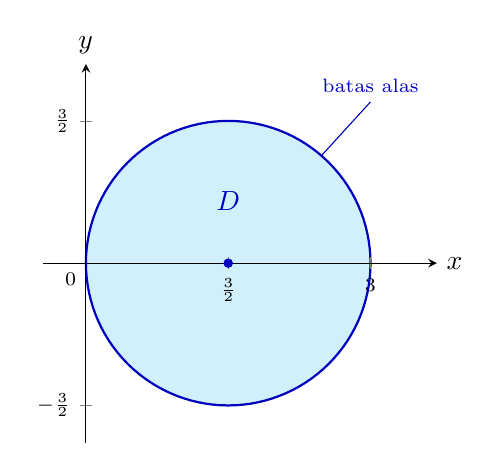
\begin{tikzpicture}
              \begin{axis}[
                  width=6.7cm,height=6.4cm,
                  axis lines=middle,axis equal image,axis on top,
                  xmin=-0.45,xmax=3.7,ymin=-1.9,ymax=2.1,
                  xlabel={$x$},ylabel={$y$},
                  xlabel style={at={(axis description cs:1,0.475)},anchor=west},
                  ylabel style={at={(axis description cs:0.108,1)},anchor=south},
                  xtick={0,1.5,3},xticklabels={$0$,$\frac32$,$3$},
                  ytick={-1.5,1.5},yticklabels={$-\frac32$,$\frac32$},
                  tick label style={font=\scriptsize},
                  clip=false,
                ]
                \addplot[draw=blue!75!black,fill=cyan!18,thick,
                  domain=0:360,samples=121,variable=\t]
                ({1.5+1.5*cos(t)},{1.5*sin(t)}) \closedcycle;
                \addplot[only marks,mark=*,mark size=1.5pt,blue!75!black]
                coordinates {(1.5,0)};
                \node[blue!75!black] at (axis cs:1.5,0.65) {$D$};
                \node[below left,font=\scriptsize] at (axis cs:0,0) {$0$};
                \draw[blue!75!black,thin] (axis cs:2.48,1.13)
                -- (axis cs:3.0,1.7)
                node[above,font=\scriptsize] {batas alas};
              \end{axis}
            \end{tikzpicture}
            \par\small Proyeksi pada bidang $xy$.
          \end{minipage}\hfill
          \begin{minipage}[c]{0.58\linewidth}
            \centering
            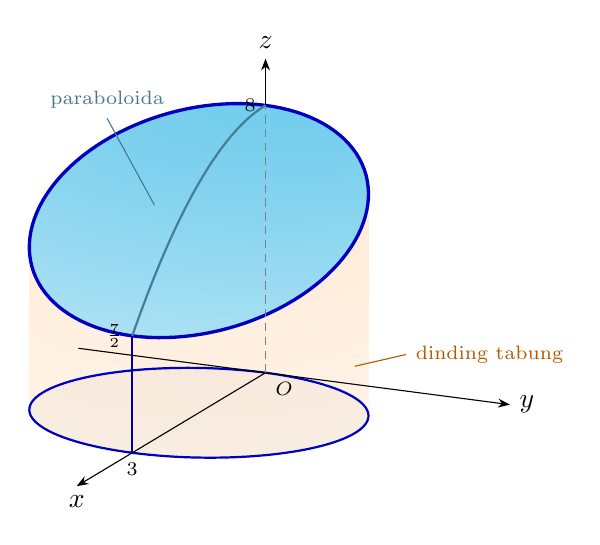
\begin{tikzpicture}
              \begin{axis}[
                  width=10.1cm,height=8cm,
                  view={115}{24},
                  axis lines=none,ticks=none,
                  xmin=-0.5,xmax=4.3,ymin=-2,ymax=2.4,zmin=0,zmax=9.5,
                  clip=false,z buffer=sort,
                ]
                % Alas: cakram pada z=0.
                \addplot3[surf,shader=interp,opacity=0.35,
                  colormap={base}{color(0cm)=(gray!20);color(1cm)=(gray!20)},
                  domain=0:1,y domain=0:360,
                  samples=13,samples y=45,variable=\r,variable y=\t]
                ({1.5+1.5*r*cos(t)},{1.5*r*sin(t)},0);
                % Dinding tabung, dari alas hingga paraboloida.
                \addplot3[surf,shader=interp,opacity=0.25,
                  colormap={wall}{color(0cm)=(orange!35);color(1cm)=(orange!65)},
                  domain=0:360,y domain=0:1,
                  samples=61,samples y=11,variable=\t,variable y=\s]
                ({1.5+1.5*cos(t)},{1.5*sin(t)},{s*(5.75-2.25*cos(t))});
                % Atap: hanya bagian paraboloida di atas cakram D.
                \addplot3[surf,shader=interp,opacity=0.78,
                  colormap={roof}{color(0cm)=(cyan!20);color(1cm)=(cyan!70)},
                  domain=0:1,y domain=0:360,
                  samples=21,samples y=61,variable=\r,variable y=\t]
                ({1.5+1.5*r*cos(t)},{1.5*r*sin(t)},
                {8-((1.5+1.5*r*cos(t))^2+(1.5*r*sin(t))^2)/2});
                \addplot3[thick,blue!75!black,domain=0:360,
                  samples=121,samples y=0,z buffer=none,variable=\t]
                ({1.5+1.5*cos(t)},{1.5*sin(t)},0);
                \addplot3[very thick,blue!75!black,domain=0:360,
                  samples=121,samples y=0,z buffer=none,variable=\t]
                ({1.5+1.5*cos(t)},{1.5*sin(t)},{5.75-2.25*cos(t)});
                \addplot3[thick,cyan!55!black,domain=0:3,
                  samples=61,samples y=0,z buffer=none]
                (x,0,{8-x^2/2});
                \addplot3[thick,blue!65!black,domain=0:1,
                  samples=2,samples y=0,z buffer=none] (3,0,{3.5*x});
                \draw[-{Stealth[length=1.5mm]},black]
                (axis cs:0,0,0) -- (axis cs:4.25,0,0) node[below] {$x$};
                \draw[-{Stealth[length=1.5mm]},black]
                (axis cs:0,-1.8,0) -- (axis cs:0,2.35,0) node[right] {$y$};
                \draw[densely dashed,gray] (axis cs:0,0,0) -- (axis cs:0,0,8);
                \draw[-{Stealth[length=1.5mm]},black]
                (axis cs:0,0,8) -- (axis cs:0,0,9.4) node[above] {$z$};
                \node[below right,font=\scriptsize] at (axis cs:0,0,0) {$O$};
                \node[left,font=\scriptsize] at (axis cs:0,0,8) {$8$};
                \node[below,font=\scriptsize] at (axis cs:3,0,0) {$3$};
                \node[left,font=\scriptsize] at (axis cs:3,0,3.5) {$\frac72$};
                \draw[cyan!50!black,thin] (axis cs:1.8,-0.3,6.335)
                -- ++(-0.6cm,1.1cm)
                node[above,font=\scriptsize] {paraboloida};
                \draw[orange!70!black,thin] (axis cs:1.5,1.5,2)
                -- ++(0.65cm,0.15cm)
                node[right,font=\scriptsize] {dinding tabung};
              \end{axis}
            \end{tikzpicture}
            \par\small Benda di atas $z=0$, di dalam tabung.
          \end{minipage}
        \end{center}

  \item Anggap $U=U(x,y)$ dan $V=V(x,y)$.
        Saat menurunkan terhadap $x$, variabel $y$ dianggap konstan.
        Dari kedua persamaan diperoleh
        \[
          \begin{cases}
            2U_x-3V_x-y+2x=0, \\
            3U_x+2V_x+y=0,
          \end{cases}
          \qquad\Longleftrightarrow\qquad
          \begin{cases}
            2U_x-3V_x=y-2x, \\
            3U_x+2V_x=-y.
          \end{cases}
        \]
        Untuk menghilangkan $V_x$, kalikan persamaan pertama dengan $2$
        dan persamaan kedua dengan $3$, lalu jumlahkan:
        \[
          13U_x=2(y-2x)+3(-y)=-4x-y.
        \]
        Untuk menghilangkan $U_x$, gunakan $-3$ kali persamaan pertama
        ditambah $2$ kali persamaan kedua:
        \[
          13V_x=-3(y-2x)+2(-y)=6x-5y.
        \]
        Jadi,
        \[
          U_x=\frac{-4x-y}{13},\qquad V_x=\frac{6x-5y}{13}.
        \]

        Selanjutnya, turunkan kedua persamaan awal terhadap $y$.
        Kali ini, $x$ dianggap konstan:
        \[
          \begin{cases}
            2U_y-3V_y-x=0, \\
            3U_y+2V_y+x-2y=0,
          \end{cases}
          \qquad\Longleftrightarrow\qquad
          \begin{cases}
            2U_y-3V_y=x, \\
            3U_y+2V_y=2y-x.
          \end{cases}
        \]
        Dengan kombinasi eliminasi yang sama,
        \begin{align*}
          13U_y & =2x+3(2y-x)=6y-x,   \\
          13V_y & =-3x+2(2y-x)=4y-5x.
        \end{align*}
        Maka keempat turunannya adalah
        \[
          \boxed{
            \begin{aligned}
              U_x & =\frac{-4x-y}{13}, & U_y & =\frac{6y-x}{13},  \\[3pt]
              V_x & =\frac{6x-5y}{13}, & V_y & =\frac{4y-5x}{13}.
            \end{aligned}}
        \]

  \item Misalkan setengah panjang sisi balok adalah $a,b,c>0$.
        Balok dapat dipilih berpusat di titik asal.
        Sebab, jika pusatnya $(h,k,\ell)$, syarat seluruh titik sudut berada
        di dalam elipsoida memberikan
        \[
          (|h|+a)^2+\frac{(|k|+b)^2}{9}
          +\frac{(|\ell|+c)^2}{4}\le1.
        \]
        Memindahkan pusatnya ke asal membuat ruas kiri tidak bertambah.
        Jadi, ukuran balok tetap dapat dipertahankan.

        Titik sudut balok yang berpusat di asal adalah $(\pm a,\pm b,\pm c)$.
        Volume dan kendalanya adalah
        \[
          V=8abc,\qquad a^2+\frac{b^2}{9}+\frac{c^2}{4}\le1.
        \]
        Pada volume maksimum, kendala harus berupa persamaan.
        Jika masih kurang dari $1$, ketiga sisi masih dapat diperbesar.

        Gunakan pengali Lagrange dengan
        \[
          \mathcal L=8abc-\lambda\left(a^2+\frac{b^2}{9}+\frac{c^2}{4}-1\right).
        \]
        Turunan terhadap $a,b,c$ memberikan
        \[
          8bc=2\lambda a,\qquad
          8ac=\frac{2\lambda b}{9},\qquad
          8ab=\frac{\lambda c}{2}.
        \]
        Kalikan masing-masing persamaan dengan $a,b,c$ secara berurutan:
        \[
          8abc=2\lambda a^2
          =\frac{2\lambda b^2}{9}
          =\frac{\lambda c^2}{2}.
        \]
        Karena $a,b,c>0$, maka $\lambda\ne0$.
        Oleh karena itu,
        \[
          a^2=\frac{b^2}{9}=\frac{c^2}{4}.
        \]
        Jumlah ketiga suku tersebut adalah $1$, sehingga setiap suku bernilai $\frac13$:
        \[
          a=\frac1{\sqrt3},\qquad b=\sqrt3,\qquad c=\frac2{\sqrt3}.
        \]
        Panjang sisi-sisi balok adalah
        \[
          2a=\frac2{\sqrt3},\qquad 2b=2\sqrt3,\qquad 2c=\frac4{\sqrt3}.
        \]
        Jadi, isi balok terbesarnya
        \[
          \boxed{V_{\max}
            =\frac2{\sqrt3}\,(2\sqrt3)\,\frac4{\sqrt3}
            =\frac{16}{\sqrt3}=\frac{16\sqrt3}{3}.}
        \]
        Nilai ini merupakan maksimum global.
        Untuk melihatnya, ambil $u=a^2$, $v=b^2/9$, dan $w=c^2/4$.
        Karena $u+v+w\le1$, ketaksamaan rata-rata aritmetika dan geometri memberi
        \[
          uvw\le\left(\frac{u+v+w}{3}\right)^3\le\frac1{27}.
        \]
        Maka $V=48\sqrt{uvw}\le16/\sqrt3$, dan kesamaan dicapai oleh ukuran di atas.
\end{enumerate}
\end{document}
